\documentclass{standalone}
\usepackage{tikz}

\begin{document}

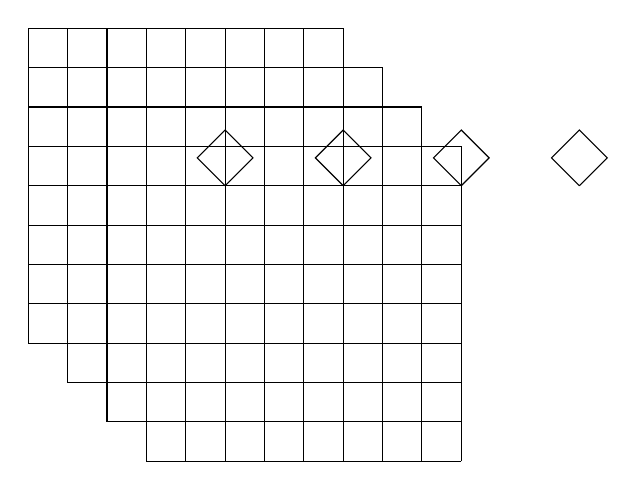
\begin{tikzpicture}[scale=0.5]
\foreach \x in {0,...,3}{
    \draw[shift={(\x,-\x)}] (-4,4) grid (4,-4);
    \draw[shift={(3*\x+1,0)}] (0,0) --++(135:1cm) --++(45:1cm)--++(-45:1cm)--++(-135:1cm);
}
\end{tikzpicture}

\end{document}